%%  siamltex.cls (main LaTeX macro file for SIAM)
%%  siamltex.sty (includes siamltex.cls for compatibility mode)
%%  siam10.clo   (size option for 10pt papers)
%%  subeqn.clo   (allows equation numbners with lettered subelements)
%%  siam.bst     (bibliographic style file for BibTeX)
%%  docultex.tex (documentation file)
%%  lexample.tex (this file)
%%
%% \CharacterTable
%%  {Upper-case    \A\B\C\D\E\F\G\H\I\J\K\L\M\N\O\P\Q\R\S\T\U\V\W\X\Y\Z
%%   Lower-case    \a\b\c\d\e\f\g\h\i\j\k\l\m\n\o\p\q\r\s\t\u\v\w\x\y\z
%%   Digits        \0\1\2\3\4\5\6\7\8\9
%%   Exclamation   \!     Double quote  \"     Hash (number) \#
%%   Dollar        \$     Percent       \%     Ampersand     \&
%%   Acute accent  \'     Left paren    \(     Right paren   \)
%%   Asterisk      \*     Plus          \+     Comma         \,
%%   Minus         \-     Point         \.     Solidus       \/
%%   Colon         \:     Semicolon     \;     Less than     \<
%%   Equals        \=     Greater than  \>     Question mark \?
%%   Commercial at \@     Left bracket  \[     Backslash     \\
%%   Right bracket \]     Circumflex    \^     Underscore    \_
%%   Grave accent  \`     Left brace    \{     Vertical bar  \|
%%   Right brace   \}     Tilde         \~}


\documentclass[final,leqno,fullpage]{siamltex}

\usepackage{jpfairbanks}
\usepackage{tabularx}
\usepackage{subfig}
\usepackage{booktabs}
% \usepackage{tabu}
% definitions used by included articles, reproduced here for 
% educational benefit, and to minimize alterations needed to be made
% in developing this sample file.

\newcommand{\pe}{\psi}
\def\d{\delta} 
\def\ds{\displaystyle} 
\def\e{{\epsilon}} 
\def\eb{\bar{\eta}}  
\def\enorm#1{\|#1\|_2} 
\def\Fp{F^\prime}  
\def\fishpack{{FISHPACK}} 
\def\fortran{{FORTRAN}} 
\def\gmres{{GMRES}} 
\def\gmresm{{\rm GMRES($m$)}} 
\def\Kc{{\cal K}} 
\def\norm#1{\|#1\|} 
\def\wb{{\bar w}} 
\def\zb{{\bar z}} 

% some definitions of bold math italics to make typing easier.
% They are used in the corollary.

\def\bfE{\mbox{\boldmath$E$}}
\def\bfG{\mbox{\boldmath$G$}}

\title{QR factorization with sparse additive updates}

% The thanks line in the title should be filled in if there is
% any support acknowledgement for the overall work to be included
% This \thanks is also used for the received by date info, but
% authors are not expected to provide this.

\author{James Fairbanks and Domenic Carr}

\begin{document}

\maketitle

\begin{abstract}
QR factorizations can be an important tool when applying least squares fits to data. However, data updates cause changes to QR factorizations, which require computation.  Often, full re-computation of a QR factorization is required via Householder transformations. When the data changes in a sparse, additive way, however, it is possible to avoid full re-computation by leveraging the specialized structure of the update.  This accelerates computation of the new QR factorization. In this paper, we detail the matrix and sparsity conditions for which specialized updating algorithms outperform full QR re-computation.
\end{abstract}

\begin{keywords} 
QR factorization, Incremental Computation, Streaming Linear Algebra.
\end{keywords}

\begin{AMS}
15A15, 15A09, 15A23
\end{AMS}

\pagestyle{myheadings}
\thispagestyle{plain}
\markboth{CSE6443}{Course Project}


\section{Introduction and examples}
This paper concerns the goal of maintaining a least squares fit with changing data. In current literature, the changes in matrix factorizations caused by low rank updates and the addition of new data points
have been studied \cite{incrementalGivens} \cite{LowrankQRupdate}. In this work, our objective is to address how the QR factorization changes resulting from sparse additive changes to the observed data and to determine when it is possible to use specialized algorithms to accelerate computing the updated QR factorization. 

We examine when $A$ is an $m\times n$ matrix with $m \ge n $. We have an update to $A$ called $\Delta A$ which has only a few nonzero columns.
This would represent a case when only a few dimensions have updates. For example, when studying the term document matrix $A_{i,j}$ represents the number of 
occurances of word $i$ in document $j$. If the $j$th document changes and thus acquires new words then $\Delta A$ will contain nonzero entries only in the $j$th column. Another example is a dynamic graph where new edges are presented and the algorithm is using a low rank representation of vertices based on $QR_k$ where $R_k$ a rank $k$ truncated version of $R$. Then, updates to $A$ are the new edges and changes in this low rank representation can be used to study the dynamics of the graph \cite{lowrankgraphrepresentations}. In both cases, we can take advantage of the special structure of $\Delta A$ to accelerate the QR decomposition of $A+\Delta A$ by leveraging the information contained in the QR factorization of $A$.

\subsection{Goals}
In this paper we present two specialized forms of the Givens rotation algorithm that perform these updates. We provide an equation counting the flops required by each method, and compare them to the standard Householder QR algorithm. 
Since these equations depend on the specific column being updated, we provide an average case analysis for randomly selected columns. We experimentally estimate the cross over point for various values of $m,n,k$ where $m$ is the number of rows, $n$ is the number of columns and $k$ is the number of updated columns.
\section{Algorithm}
We exploit a key structure in this problem. If $X = xe_i^T$ for some vector $x\in \R^m$ and $Q$ is a matrix in $\R^{m\times n}$ then $Q^TX$ has nonzero entries only in the $i$th column.
This implies that updates to any number of data elements in the same dimension will incur the same number of nonzero entries when attempting to update the QR factorization.
We also leverage Givens rotations to selectively eliminate entries of a matrix while creating the orthogonal transformation $Q$ and upper triangular factor $R$.
This selectivity allows us to use Givens rotations in a way that we could not use Householder transformations. For example, consider the case when the $i$th column of $A$ contained nonzero elements.  Applying a single Householder transformation
on the $ith$ dimension would create fill-in entries in potentially every element in columns $i$ through $n$, completely nullifying our sparsity structure. Consequently, this would require performing $n-i$ transformations to restore the damage caused by changing the $ith$ column.

In contrast, the Givens rotations allow us to selectively eliminate entries of the matrix with only minor fill-in penalties, which vary based on the order and location of Givens rotations. The next section will detail various rotation-ordering algorithms, count the fill-in introduced by each ordering, and determine the algorithm that incurs the smallest fill-in penalty.
\section{Annihilation Ordering}
When considering how to order our Givens rotations, we must decide whether to go row-wise or column-wise and  whether to annihilate entries from top-down or from bottom-up.
We first examine row-wise operation. If we eliminate from top to bottom row-wise, we will introduce zeros in the entire row by eliminating against row $1$.
%This fact can be proved inductively.
Eliminating the original entries of row $j$ will introduce fill-in in all of row $j$.
If we go from bottom to top, then we introduce oscillatory fill-in.
Eliminating entry $m,i_2$ will introduce a zero in entry $m,i_1$ and vice versa. This indicates that we should operate column-wise. 

When operating column-wise, if we eliminate entries from the left-most nonzero column, we introduce fill-in entries on the first off-diagonal of the entire matrix. We then eliminate the fill-in entries between the left-most nonzero column (which has now been zeroed) and then next leftmost nonzero column.
This incurs the cost of eliminating $i_{j+1}-i_{j}$ fill-in entries. We then eliminate column $i_{j+1}$ which introduces another off-diagonal of fill-in entries.
The total number of fill-in entries eliminated is 
\[ Lazy = \sum_{j=1}^k \sum_{t=1}^j (i_{j+1} - i_{j} - t) = \sum_{j=1}^k j(i_{j+1}-i_{j} - \frac{j+1}{2})
\]
We call this the lazy elimination strategy because we defer elimination of fill-in entries until the last possible moment.

An alternative strategy is to eliminate fill-in as soon as it is created. We call this the eager elimination strategy. We eliminate column $i_j$ and this fills in the first off-diagonal. Then before eliminating column $i_{j+1}$ we annihilate the first off-diagonal entries. Then, when eliminating column $i_{j+1}$ we reintroduce fill-in on the first off-diagonal between columns $i_{j+1}$ and $n$.
The total number of fill-in entries removed is
\[ Eager = \sum_{j=1}^k j(n - i_{j}) = n\sum_{j=1}^k j - \sum_{j=1}^k ji_j = \frac{nk(k+1)}{2} - \sum_{j=1}^k i_j
%\sum_{j=1}^k n-i_j + \sum_{j=1}^k j(i_{j+1}-i_{j} - \frac{j+1}{2}
\]
Both methods must eliminate the original nonzeros which are counted by $\sum_{j=1}^k n-i_j $. 
\begin{align}
Eager-Lazy &= \sum_{j=1}^k nj - \sum_{j=1}^k ji_j - \sum_{j=1}^k j(i_{j+1}-i_{j} + \frac{j+1}{2}) \\
& = \sum_{j=1}^k nj - \sum_{j=1}^k j(i_{j+1} + \frac{j+1}{2})
\end{align}
Since $n\ge i_{j+1}$ for all $j$, we conclude that the lazy strategy is more efficient than the eager strategy. That is, the lazy elimination strategy requires fewer eliminations.
The primary reason is because the lazy strategy eliminates the $k$ off-diagonals while the eager strategy eliminates the first off-diagonal $k$ times. Since the $i$th off-diagonal has $n-i$ elements, there are fewer fill-in entries for the lazy method to eliminate.  Thus, it is more efficient.
%\sum_{j=1}^k n-i_j +

\subsection{Another interpretation of the eager method}
We will now explain the eager method using an alternative definition. Suppose that $\Delta A = \sum_{j=1}^k A_j$ where each $A_j$ has nonzero entries only in the $i_j$th column. That is $A_j = xe_{i_j}^T$
Then we can apply $k$ single-column updates. We make use of the equations 
\begin{align*}
Q^TA_1 + R &= Q_1 R_1 \\
Q_1^TA_2 + R_1 &= Q_2 R_2 \\
\vdots\\
Q_{k-1}^TA_k + R_{k-1} &= Q_k R_k 
\end{align*}

If we iteratively add one column at a time, then Givens rotations allows us to compute $Q_{j+1}, R_{j+1}$ from $Q_j,R_j+Q_jA_{j+1}$.
This requires $m-i_j$ rotations to eliminate the one column and fills in one off-diagonal with $n-i_j$ elements. 
This gives 
\[6(n-i_j)(m-i_j) + 6(n-i_j)(n-i_j)\]
flops to perform the rotations and
\[6n(m-i_j) + 6n(n-i_j)\]
flops to update $Q$
Each iteration also requires a single, dense matrix-vector product because we must compute $Q_j^TA_{j+1} + R_j$
We must perform this $k$ times. 

When examining this method, we see that performing the factorization
\[Q_{k-1}^TA_k + R_{k-1} = Q_k R_k \]
 introduces the fill-in entries and immediately eliminates them. This recovers the eager strategy discussed earlier.
\todo[inline]{Should we present this interpretation first?}

\section{Comparison to Householder QR factorization}\label{sec:compare}
From Golub and Van Loan, the required flop count for the Householder reflection method when accumulating the orthogonal basis $Q$ is $4(m^2n - mn^2 +n^3/3) + 2(n^2m - n/3)$. 
We know that the static Givens rotations method takes $6mn(n+1)/2 + 6mn^2$ to accumulate the orthogonal matrix $Q$. 
Our method depends on the particular columns perturbed by the update, which leads to a more complicated formula. 
Let $(\cdot)^+$ be the function $max(\cdot, 0)$.
For the sparse update we use at most
\[
  \sum_{j=1}^k 6(n-i_j)(m-i_j) + 6(n-i_{j})^{+}
\]
flops for eliminating the fill-in. This value is an upper bound because when counting the flops for eliminating the fill-in entries, we count all of the fill-in entries that are in the $j$th gap, as if they are at the position $(i_{j+1},i_j)$. These flops are also accompanied by the flops necessary to update $Q$, which are counted as

\[
  \sum_{j=1}^k 6n(m-i_j) + 6nj\left(i_{j+1}-i_{j} + \frac{j+1}{2}\right)
\]

We can compare the flop counts of full re-computation with our sparse update methods. For the purpose of analytic tractability we will use the eager method and make use of order of growth bounds.
Under the assumption that $m\ge n$ and $m\approx m-1, n\approx n-1$ $k=1$ and $i_1=1$
\begin{align*}
T_{eager}(m,n,k) &= 6(n-1)(m-1) + 6(n-1)(n-1) + 6n(m-1) + 6n(n-1) + m^2\\
    &\approx 12(nm+n^2) + m^2
\end{align*}
We can thus suppose that we are making $k$ updates to an $m,n$ matrix. We bound the cost of this operation by the $k$ times the cost to update the first column, which is the most expensive column to update.
Thus, we can derive a lower bound on the ratio of $T_{full}$ to $T_{eager}$.

\begin{align}\label{eqn:ratio}
  \frac{T_{full}}{T_{eager}}(m,n,k) &\ge \frac{4m^2n - 4mn^2 + 4n^3/3 + 2n^2(m-n/3)}{12k(nm+n^2) + km^2}\\
        &\ge \frac{4m^2n - 2mn^2 + 2n^3/3}{12(nm+n^2) + m^2}
        %&\ge \frac{m^2n}{3k(nm+n^2) + km^2/4} - \frac{2mn^2}{12k(nm+n^2) + km^2} + \frac{2n/3}{12k(m/n+n) + k(m/n)^2}
\end{align}

For a fixed $m$ large enough, the Householder based methods are cubic in $n$, while the sparse updating methods are quadratic in $n$ because we need to accumulate $Q$. 
By making this simplification we can model the performance ratio as
\begin{equation}\label{eqn:model}
    r_e(m,n,k) = \frac{C_m n^3}{n^2k} = \frac{Cn}{k}
\end{equation}
The relationship between $m$ and $n$ is accounted for in the dependence of $C_m$ on $m$. This model is useful for understanding the experimental results below.
We see that as $n$ increases the performance ratio should increase for a fixed $k$; for a fixed $n$ the performance ratio is inversely proportional to $k$.
From Equation~\ref{eqn:ratio} we can see that as $m$ increases for a fixed $n,k$ pair the proportionality parameter $C_m$ should increase.
When $r_e=1$, the two methods will require the same amount of time. The $k$ value for which this occurs is called the break even point.
The model described by Equation\ref{eqn:model} can produce a prediction about the break even point by solving $C_mn/k = 1$, that is, $C_mn = k$.
Applying $C_{m}$ is increasing in $m$, this relationship indicates that the break even point will increase as the size of the matrix increases. We verify this experimentally in the next section.


%\frac{4m^2n - 4mn^2 + 4n^3/3 + 2n^2(m-n/3)}{m^2k + n^2k} &= C_1\frac{n + m-n}{k + (m/n)^2k} + C_2\frac{m^2n-mn^2}{m^2k + n^2k}\\
%    &= C_1\frac{n + m-n}{k + (m/n)^2k} + C_2\frac{n-n^2}{k + (n/m)^2k}\\
%    &= C_1
\section{Testing}
Our input space has three dimensions: the number of rows of $A$, $m$; the number of columns of $A$, $n$; and, the number of nonzero columns in $\Delta A$, $k$.  We examined values of $m$ of 100, 500, and 1000.  Based on the value of $m$, we chose the values of $n$ and $k$ from the following sets:
\begin{align*}
    n \in &\{ 2^i \mid 1\le i \le \log{\left(m\right)}\}\\
    k \in &\{ 2^i \mid 1 \le i \le \log{\left(n/2\right)}\}
\end{align*}
Altogether, this resulted in over 100 distinct combinations of $(m,n,k)$.  To compare each algorithm's runtime for a $(m,n,k)$~combination, we applied the following testing procedure:

For given values of $m$, $n$, and $k$,
\begin{enumerate}
\item Generate a random $m\times n$ matrix $A$
\item Generate $k$ vectors uniformly from $\R^k$
\item Place the $k$ vectors into random columns of $\Delta A$
\item Execute each QR Algorithm on $A$+$\Delta A$	
\item Repeat Steps (1)-(4) 30 times collecting the runtime
\item Determine median runtime 
\item Perform Signed-Rank Test to determine statistical significance
\end{enumerate}
The signed rank test indicates whether the difference of the two median runtimes is distinct. This is important because the runtime of the methods depends on the positions of the perturbations.
We implemented the three algorithms in Matlab and performed all testing on a laptop computer with an Intel i7 processor operating at 2.2 GHz.

\section{Results and Discussion}

After computing $t_{full}$, $t_{eager}$ and $t_{lazy}$, the median runtime for each algorithm, we investigated the ratios of algorithm runtimes for various cross-sections in our data.  The most interesting ratios were

\[r_l(m,n,k) = \frac{t_{full}(m,n,k)}{t_{lazy}(m,n,k)}
\textrm{\hspace{1cm}and\hspace{1cm}}
r_e(m,n,k) = \frac{t_{full}(m,n,k)}{t_{eager}(m,n,k)}\]
Whenever these ratios are greater than 1, the specialized updating algorithms perform better than re-computing the QR factorization using Householder transformations. Once these ratios become less than 1, however, it is more advantageous to re-compute the QR factorization. In Figure~\ref{fig:1000plot} (left), we plot $r_e (m,n,k)$ versus $\log{k}$ for fixed values of $n$\footnote{This perspective is useful when the data vectors are of a fixed dimension and a practitioner is determining how columns can be altered in one batch before recomputation is more efficient than updating.  }. From these plots, we see that as $\log{k}$ increases, $r_e$ decreases for fixed $n$.  Specifically, we see a negative linear relationship, which confirms the inverse proportionality we anticipated in Section~\ref{sec:compare}\footnote{ We only show $r_e$ since the eager method is easier to compare to its analytic model}.

On these plots we also include a line called {\texttt breakeven}, which indicates when $r_e$ is equal to 1. All points above this line imply the lazy updating algorithm is faster, while all points below this line imply the Householder algorithm is faster.  By comparing the $r_e$ curves to the breakeven line, we see that the breakeven $k$ value increases as $n$ increases.  We also see that as $m$ increases (successively lower plots), the curves shift up and to the right, indicating improved performance of the lazy algorithm.  For example, the $n=64$ curve crosses the breakeven line at $log(k) = 1.25$ for $m = 100$; at $\log(k) = 2.6$ for $m = 500$; and, at $\log(k) = 2.8$ for $m =1000$.  This tells us that the breakeven $k$ value increases as $m$ increases, for fixed $n$.  Thus, we have experimentally shown what we had predicted in Section~\ref{sec:compare}: as the matrix size increases in either dimension, the breakeven point increases.

Another perspective is determining for a fixed batch size $k$, how much faster is updating only that batch compared to the entire factorization as a function of the dimensionality of the problem $n$. We show this type of perspective in the plots of Figure~\ref{fig:1000plot} (right).  Here, we plot $r_e (m,n,k)$ versus n for fixed values of $k$. We see that there is nearly linear growth in $r(m_0, n, k_0)$ as $n$ increases, when $m$ is large. This is what we would expect from the analytic bounds on flop counts, as detailed in Section~\ref{sec:compare}. We also see that as m increases, (successively lower plots), the curves shift upward for a fixed combination of n, k.  For example, for $m=100$, the $k=1$ curve has an $r_e$ value of $5.5$ at $n = 100$; for $m=500$, the $k=1$ curve has an $r_e$ value of $22$ at $n = 500$; and, for $m=1000$, the $k=1$ curve has an $r_e$ value of 32 for $m =1000$.  Thus, as $m$ increases for a fixed $n,k$ pair, the $C_m$ value increases, which corroborates our theory from Section~\ref{sec:compare}.  We provide the tables that contain all of the data used to construct the plots in Figure~\ref{fig:1000plot} (left and right) in Figure~\ref{table:sfm}.

\newcommand{\plotwidth}{2.5in} %width of the plots in the tabular below
%insert the plots of crossover points and speedup ratios
\begin{figure}
\begin{tabular}{cc}
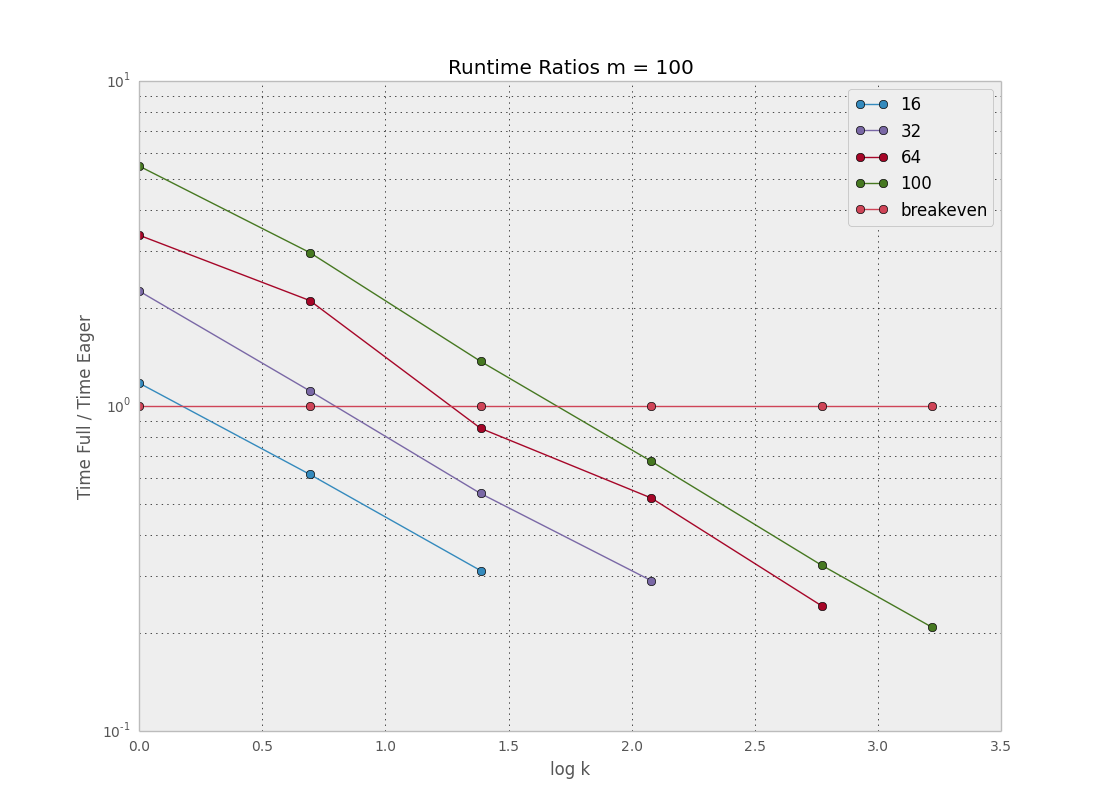
\includegraphics[width=\plotwidth]{tratio100.png} & 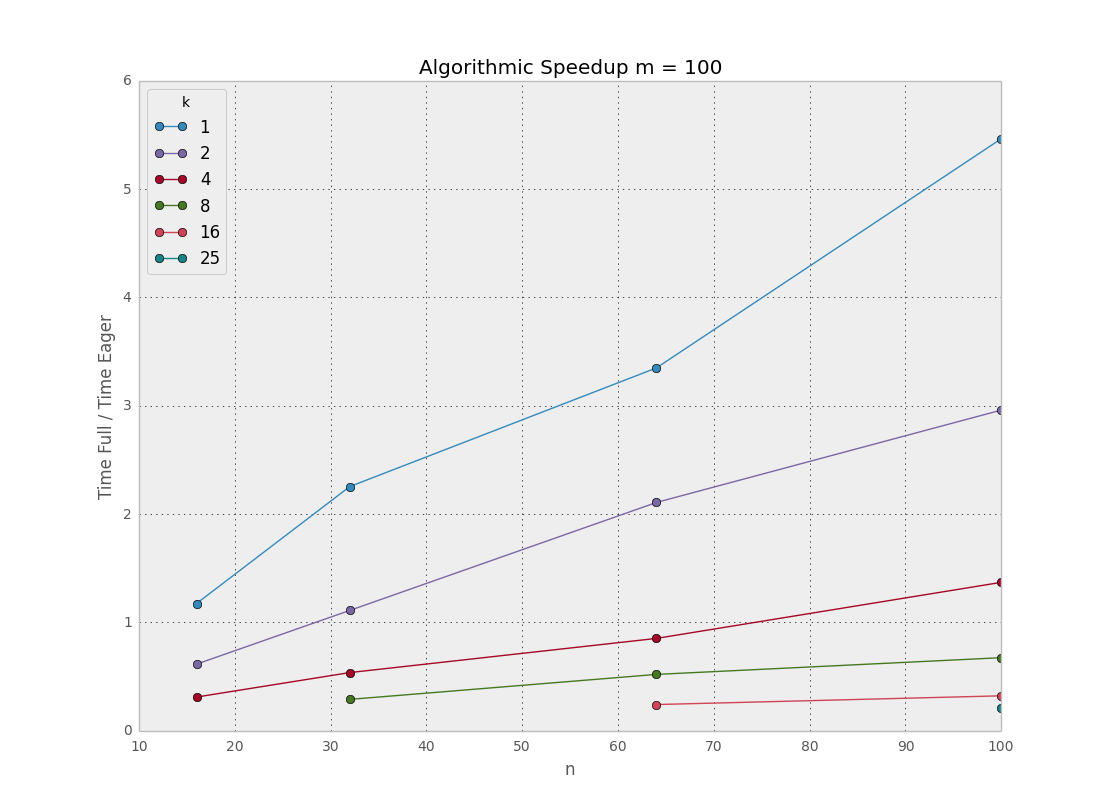
\includegraphics[width=\plotwidth]{tratioarc100.png} \\
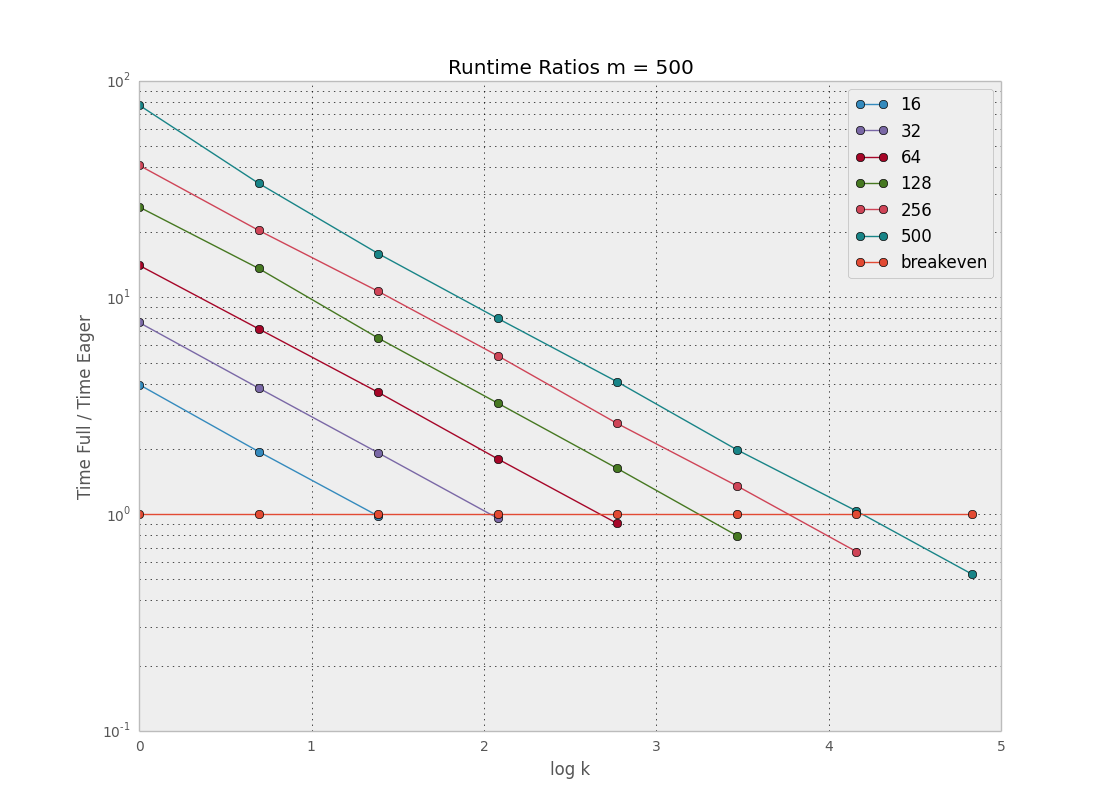
\includegraphics[width=\plotwidth]{tratio500.png} & 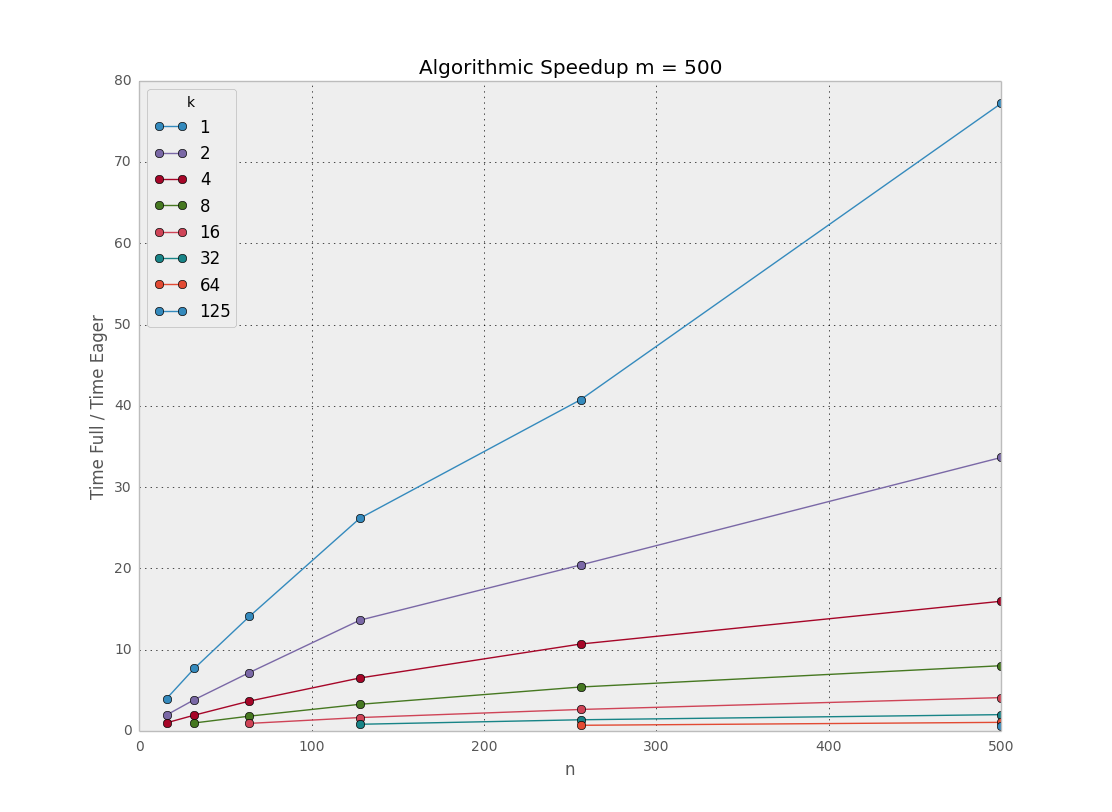
\includegraphics[width=\plotwidth]{tratioarc500.png} \\
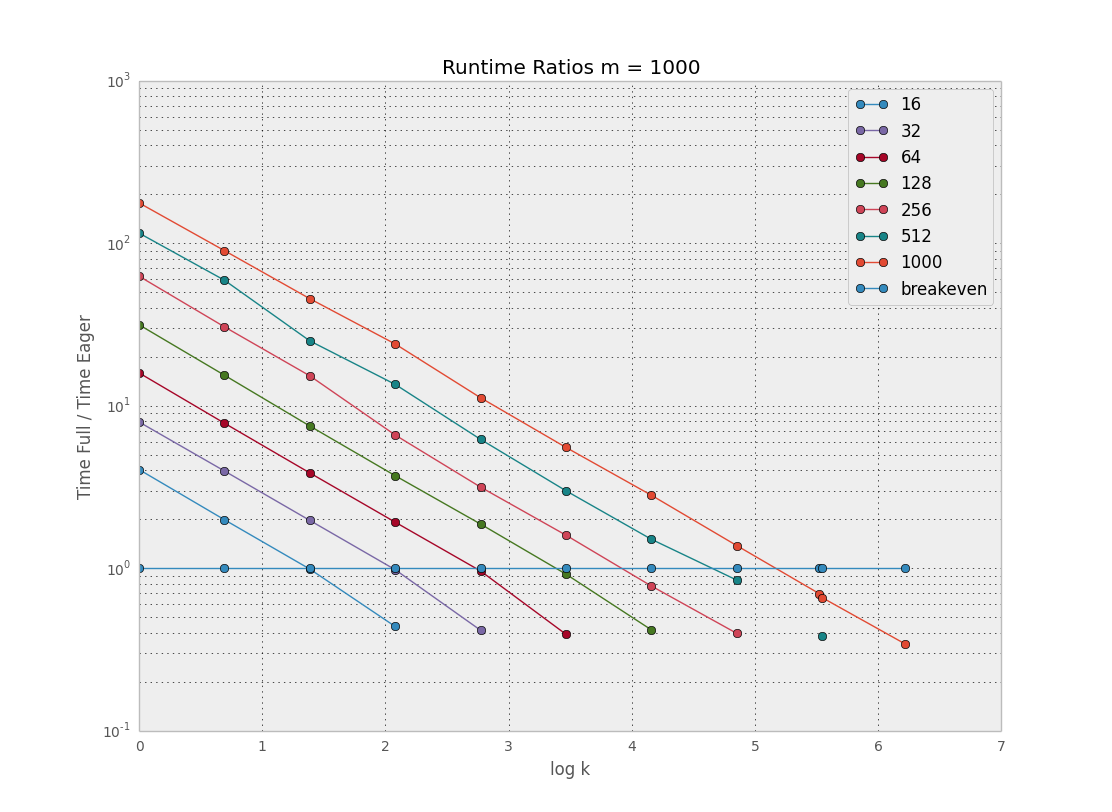
\includegraphics[width=\plotwidth]{tratio1000.png} & 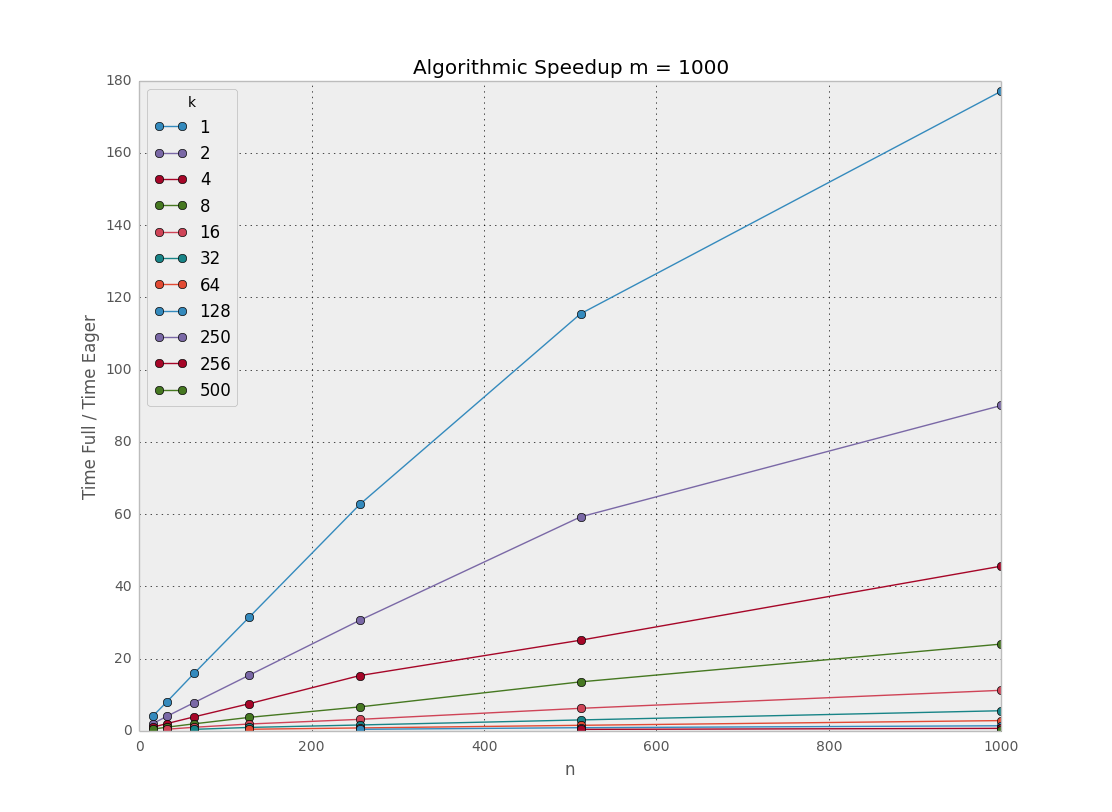
\includegraphics[width=\plotwidth]{tratioarc1000.png}\\
\end{tabular}
\caption{$r_e$ as a function of $k$ (left) and as a function of $n$ (right) }
% \label{fig:100plot}
% \label{fig:500plot}
\label{fig:1000plot}
\end{figure}
%insert the tables that have the speedup frames.
\begin{figure}
\centering
% tables produced by ls sfm* | xargs -I % -n 1 sed s/NaN/---/g % | cat > tables.tex
\begin{tabular}{lrrrr}
\toprule
{n} &       16  &       32  &       64  &       100 \\
\midrule
k  &           &           &           &           \\
1  &  1.174464 &  2.254186 &  3.348890 &  5.464774 \\
2  &  0.614962 &  1.110850 &  2.107137 &  2.959988 \\
4  &  0.311029 &  0.537040 &  0.852289 &  1.369830 \\
8  &       --- &  0.289581 &  0.520050 &  0.674347 \\
16 &       --- &       --- &  0.241873 &  0.322460 \\
25 &       --- &       --- &       --- &  0.208223 \\
\bottomrule
\end{tabular}

\begin{tabular}{lrrrrrr}
\toprule
{n} &       16  &       32  &        64  &        128 &        256 &        500 \\
\midrule
k   &           &           &            &            &            &            \\
1   &  3.963033 &  7.662772 &  14.071474 &  26.146007 &  40.734077 &  77.218781 \\
2   &  1.942927 &  3.820333 &   7.162948 &  13.604650 &  20.400014 &  33.636736 \\
4   &  0.979985 &  1.917975 &   3.650417 &   6.493244 &  10.671382 &  15.939933 \\
8   &       --- &  0.956929 &   1.798891 &   3.253542 &   5.382873 &   8.006895 \\
16  &       --- &       --- &   0.905242 &   1.624700 &   2.619620 &   4.078864 \\
32  &       --- &       --- &        --- &   0.796405 &   1.351518 &   1.983535 \\
64  &       --- &       --- &        --- &        --- &   0.671680 &   1.034494 \\
125 &       --- &       --- &        --- &        --- &        --- &   0.529203 \\
\bottomrule
\end{tabular}

\begin{tabular}{lrrrrrrr}
\toprule
{n} &      16   &      32   &       64   &       128  &       256  &        512  &        1000 \\
\midrule
k   &           &           &            &            &            &             &             \\
1   &  4.049259 &  7.944472 &  15.926325 &  31.507983 &  62.678462 &  115.458813 &  177.113035 \\
2   &  1.988675 &  3.967780 &   7.810222 &  15.412376 &  30.590654 &   59.224599 &   90.073101 \\
4   &  0.988316 &  1.969736 &   3.860258 &   7.504782 &  15.280334 &   25.072342 &   45.581149 \\
8   &  0.438223 &  0.979623 &   1.921544 &   3.711172 &   6.605146 &   13.536398 &   24.000350 \\
16  &       --- &  0.415439 &   0.961914 &   1.870153 &   3.157265 &    6.211023 &   11.198788 \\
32  &       --- &       --- &   0.392416 &   0.920219 &   1.598431 &    2.998286 &    5.543048 \\
64  &       --- &       --- &        --- &   0.417919 &   0.777768 &    1.508442 &    2.815094 \\
128 &       --- &       --- &        --- &        --- &   0.397742 &    0.845979 &    1.379412 \\
250 &       --- &       --- &        --- &        --- &        --- &         --- &    0.698539 \\
256 &       --- &       --- &        --- &        --- &        --- &    0.381570 &    0.659975 \\
500 &       --- &       --- &        --- &        --- &        --- &         --- &    0.343848 \\
\bottomrule
\end{tabular}


\caption{Tables of $r_e$ for $m=100,500,1000$ dashes indicate the test was not run}
\end{figure}

\begin{figure}
\centering
\begin{tabular}{lrrr}
\toprule
{m} &      100  &       500  &        1000 \\
\midrule
16   &  1.216168 &   3.922943 &    3.871414 \\
32   &  2.235173 &   7.657692 &    7.648598 \\
64   &  3.800537 &  14.374808 &   15.051345 \\
100  &  5.437297 &        --- &         --- \\
128  &       --- &  26.139462 &   29.736792 \\
256  &       --- &  42.204666 &   55.022052 \\
500  &       --- &  66.675017 &         --- \\
512  &       --- &        --- &  104.479743 \\
1000 &       --- &        --- &  178.217056 \\
\bottomrule
\end{tabular}


\caption{Experimentally determined breakeven points for $m=100,500,1000$. Dashes indicate the test was not run.}
\end{figure}

\begin{figure}
\centering
% tables produced
%% tables of lower and upper bounds on the breakeven points
\begin{tabular}{lrrrrrr}
\toprule
{m} &  100  &  500  &  1000   &  100  &  500  &  1000\\
\midrule
n    &       &       &       &     &       &       \\
16   &     1 &     2 &     2 &   2 &     4 &     4 \\
32   &     2 &     4 &     4 &   4 &     8 &     8 \\
64   &     2 &     8 &     8 &   4 &    16 &    16 \\
100  &     4 &   --- &   --- &   8 &   --- &   --- \\
128  &   --- &    16 &    16 & --- &    32 &    32 \\
256  &   --- &    32 &    32 & --- &    64 &    64 \\
500  &   --- &    64 &   --- & --- &   125 &   --- \\
512  &   --- &   --- &    64 & --- &   --- &   128 \\
1000 &   --- &   --- &   128 & --- &   --- &   250 \\
\bottomrule
\end{tabular}

\caption{Tables of bounds on the $k$ where $r_e=1$. lower bounds (left) followed by upper bounds (right), dashes indicate the test was not run}
\end{figure}

As detailed in Section~\ref{sec:compare}, the model described by Equation~\ref{eqn:model} can produce a prediction of the breakeven point by solving $C_m n = k$.  As described previously, we can determine $C_m$ experimentally from our data, and then use this value to predict where the breakeven point will occur.  Figure~\ref{table:keven} contains a table of experimentally determined breakeven points by using this method.  Comparing these values to their counterparts in Figure~\ref{table:bounds}, which contains our analytic model's lower and upper bound predictions for the breakeven points, we see that all of our experimental results fall within the bounds predicted by our analytic model.


Since the analysis of the eager method is simpler, we present mostly the results of the eager code. However since the flop count of the lazy method is lower, it outperforms the eager method. This can be verified in Table~\ref{table:sle} which shows $\frac{T_{eager}(500,n,k)}{T_{lazy}(500,n,k)}$. The signed rank test results for $m=500,k=1$ indicate that for small $k$ and small $n$ lazy and eager cannot be distinguished in run time. But for large $n$ and small $k$ eager is faster than lazy. This confirms out expectation because  $\sum_{i=1}^k n-i \approx kn$ but simpler code gives the eager method an advantage, but when $k$ is large, the approximation does not hold.

\section{Conclusion}
In this paper, we have shown how specialized algorithms can improve the performance of QR factorization updating under sparse additive updates.  We presented an analytic model for the performance gains. We used this model to predict the anticipated performance increase for various conditions.  Upon implementing the algorithms and comparing their performances experimentally, we corroborated the theory we had presented.

%\newpage{}
\begin{thebibliography}{10}

\bibitem{Golub-VanLoan}
{\sc G.~H. Golub and C.~F. Van~Loan}, {\em Matrix Computations}, 
  Second ed., The Johns  Hopkins University Press, Baltimore, MD,  1989.

\bibitem{daniel-james}{\sc Daniel, James W., et al.}, {\em Reorthogonalization and stable algorithms for updating the Gram-Schmidt QR factorization.} in Mathematics of Computation 30.136 (1976): 772-795.

\bibitem{gill1976}{\sc Gill, Philip E., et al.}, {\em Methods for modifying matrix factorizations.} Mathematics of Computation 28.126 (1974): 505-535.

\end{thebibliography} 

\end{document} 

% article{daniel1976reorthogonalization,
%   title={Reorthogonalization and stable algorithms for updating the Gram-Schmidt 𝑄𝑅 factorization},
%   author={Daniel, James W and Gragg, Walter Bill and Kaufman, Linda and Stewart, GW},
%   journal={Mathematics of Computation},
%   volume={30},
%   number={136},
%   pages={772--795},
%   year={1976}
% }

% @article{gill1974methods,
%   title={Methods for modifying matrix factorizations},
%   author={Gill, Philip E and Golub, Gene H and Murray, Walter and Saunders, Michael A},
%   journal={Mathematics of Computation},
%   volume={28},
%   number={126},
%   pages={505--535},
%   year={1974}
% }
